\documentclass[11pt]{article}
\usepackage[croatian]{babel}  % Croatian typographical rules and hyphenation patterns
\usepackage[utf8]{inputenc}  	% Encoding of Croatian characters
\usepackage[T1]{fontenc}
\usepackage{ae,aecompl}     	% Type 1 fonts, similar to Computer Modern

\usepackage{microtype}				% Improves spacing

\usepackage{booktabs}					% Nice looking tables
\usepackage{enumerate}				% Additional options for listing of items in enumerate environment
\usepackage{algorithm2e}			% Writing pseudo-code
\usepackage{todonotes}				% Adding todo items
\usepackage{dirtree}					% Simple display of directory tree
\usepackage{hyperref}
\usepackage{graphicx}
\usepackage{subfig}
\usepackage{caption}
\usepackage{listings}

\graphicspath{ {./images/} }

\hypersetup{
    colorlinks=true,
    linkcolor=blue,
    filecolor=magenta,
    urlcolor=cyan,
}
\urlstyle{same}
\usepackage{graphics}
\title{
	\Large Sveučilište Josipa Jurja Strossmayera u Osijeku \\
	Fakultet elektrotehnike, računarstva i informacijskih tehnologija \\
	\vspace{4cm}
	\Large Kolegij: Linux u ugradbenim sustavima \\
	\vspace{4cm}
	\Large \textbf{Laboratorijska vježba 2:\\Upoznavanje s Raspberry Pi 3
	računalom. Izgradnja Linuxa za Raspberry Pi 3}
	}
\date{}
\begin{document}
\maketitle
\thispagestyle{empty}
\newpage

\section{Uvod}
Na tržištu se početkom 2012. godine pojavilo računalo Raspberry Pi i pokrenulo
 malu revoluciju u području obrazovanja i hobija vezanih za računalne znanosti.
 Ovo računalo je postalo izrazito popularno zbog svoje cijene (oko 35\$) i
 malih dimenzija (8,6cm x 5,4cm x 1,7cm). Iako je Raspberry Pi računalo opće
 namjene, ima mogućnost priključivanja različite opreme (npr. različiti senzori
 i aktuatori) pa se koristi u mnogim hobi projektima u području ugradbenih
 računalnih sustava i interneta objekata, a sve češće i u različitim
 komercijalnim projektima. Glavni dio ovog računala predstavlja SoC (engl.
 \textit{System On a Chip}) uz koji se nalazi različita periferija poput RAM
 memorije, HDMI izlaza, Ethernet priključka i sl. Također, na pločici se
 nalaze i pinovi koji predstavljaju ulazno izlazne pinove opće namjene (engl.
 \textit{General Purpose Input Output - GPIO}) koji omogućuje spajanje, u
 svijetu PC-a, nestandardne opreme.

\section{Modeli Raspberry Pi računala}
Do danas je na tržište izašlo nekoliko generacija Raspberry Pi računala.
Svima je zajednički Broadcom SoC s integriranim ARM procesorom (CPU) i
 ugrađenim grafičkim procesorom (GPU).
Brzina takta procesora se kreće od 700 MHz do 1.4 GHz kod modela Pi 3B+ ili
 1.5 GHz kod modela Pi 4. Količina memorije (RAM) se kreće od 256 MB do 1 GB
 ili čak 4 GB kod najjačeg modela najnovijeg Pi 4. \textit{Secure Digital} (SD)
 kartice se koriste za pohranu operativnog sustava i programa. Na pločama se
 nalaze do četiri USB priključka. Za video izlaz koristi se HDMI.
 Pomoću GPIO pinova podržani su standardni protokoli kao što je
 I\textsuperscript{2}C.
Svi B modeli imaju \textit{Ethernet} priključak, dok modeli Pi 3 i Pi Zero W
imaju \textit{Wi-Fi 802.11n} te \textit{Bluetooth}.
\newline
\newline
\textbf{Raspberry Pi Zero} manjih dimenzija i s reduciranim brojem
 ulazno-izlaznih jedinica te ulazno-izlaznih jedinica opće namjene (GPIO) je
 izašao na tržište 2015. godine s cijenom od 5\$. 2017. godine izlazi
 \textbf{Raspberry Pi Zero W} s dodanim \textit{Wi-Fi} i \textit{Bluetooth}
 mogućnostima.
\begin{figure}[h!]
\centering
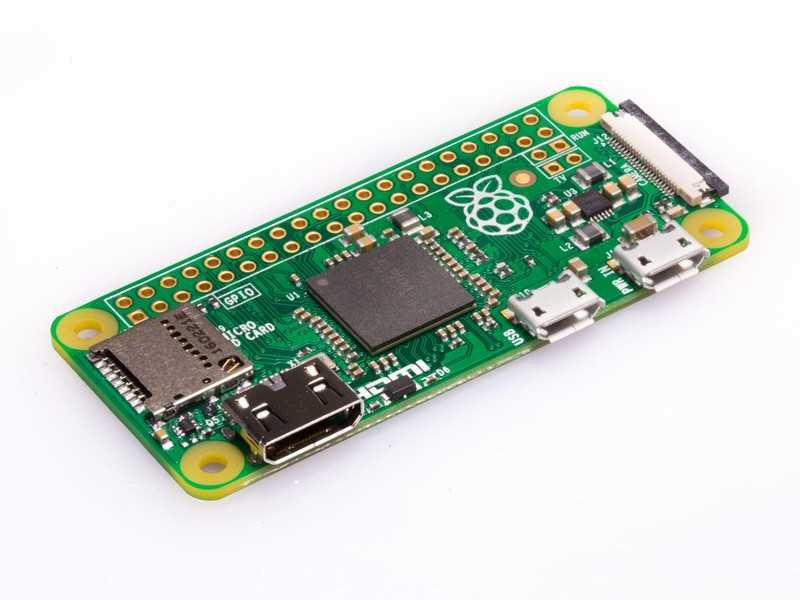
\includegraphics[width=0.8\textwidth]{rpi-zero.jpg}
\captionsetup{justification=centering}
\caption{Raspberry Pi Zero}
\end{figure}
\newline
\textbf{Raspberry Pi 3 Model B} je izašao 2016. godine s 1.2 GHz 64-bitnim
 četverojezgrenim procesorom te ugrađenim 802.11n Wi-Fi i Bluetooth mrežnim
 mogućnostima. 2018. godine izlazi \textbf{Raspberry Pi 3 Model B+} s 1.4 GHz
 procesorom te gigabitnom \textit{Ethernet} mrežom ne punih mogućnosti (u
 stvarnim testovima dostiže brzinu 300 Mbit/s, jer dijeli USB 2.0 sabirnicu).
 Posjeduje \textit{dual-band 802.11ac 2.4/5 Ghz Wi-Fi} bežični mrežni standard.
\newline
 Najnoviji model izlazi 2019. godine. Radi se o modelu \textit{Raspberry Pi
 4 Model B}. Hardverski definitivno najjači model Raspberry Pi računala s
 1.5 GHz četverojezgrenim \textbf{ARM Cortex-A72} procesorom, podrškom za
 802.11ac Wi-Fi bežičnom mrežom, \textbf{Bluetooth 5} podrškom,
 podrškom za gigabitnom Ethernet mrežom punih mogućnosti, dva \textbf{USB 2.0}
 porta, dva \textbf{USB 3.0} porta te podrškom za \textbf{4K} video rezolucijom.
\begin{figure}[h!]
\centering
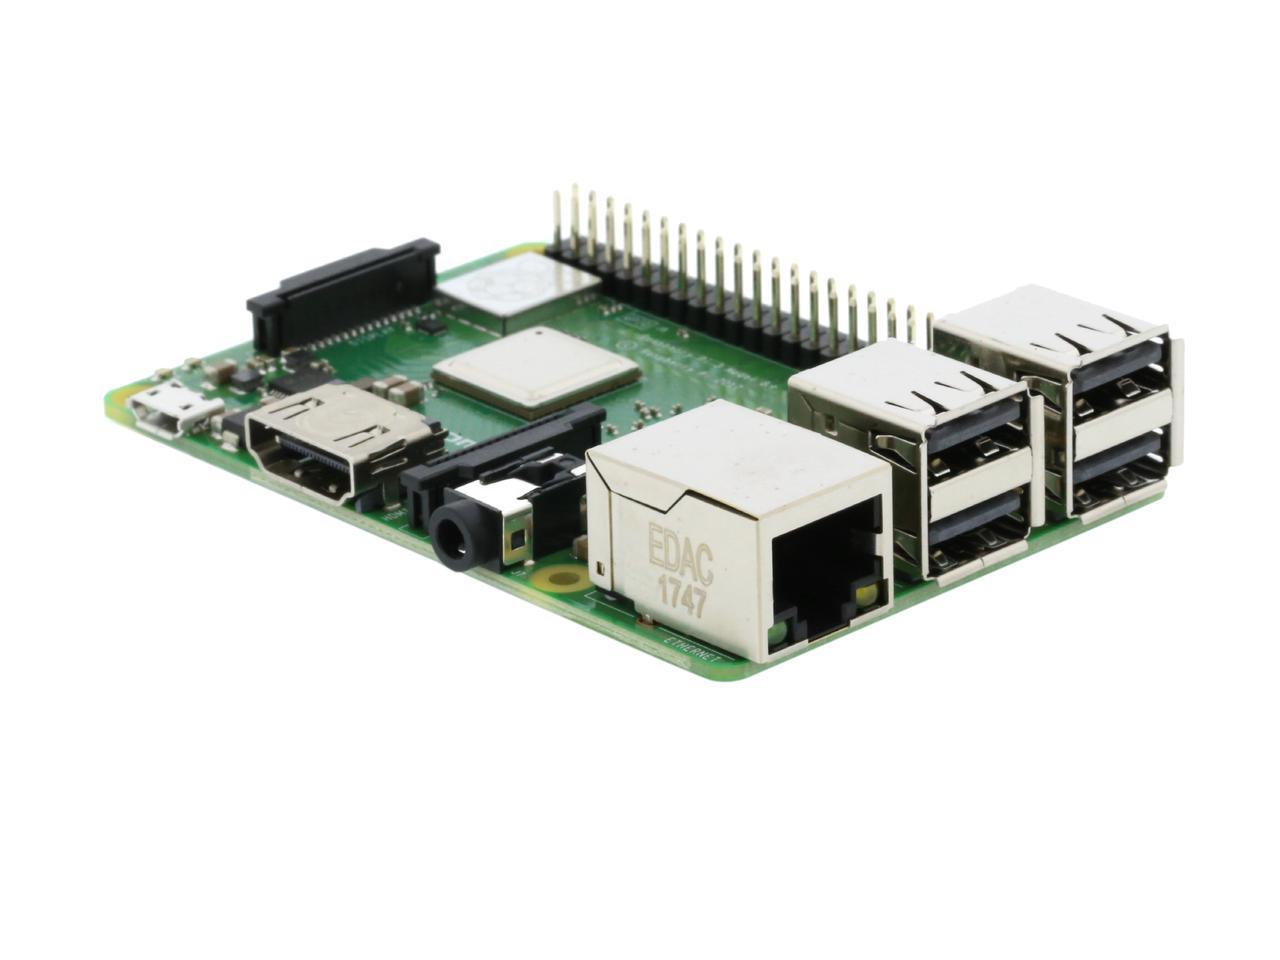
\includegraphics[width=0.8\textwidth]{rpi-3-b-plus.jpg}
\captionsetup{justification=centering}
\caption{Raspberry Pi 3 B+}
\end{figure}
\begin{figure}[h!]
\centering
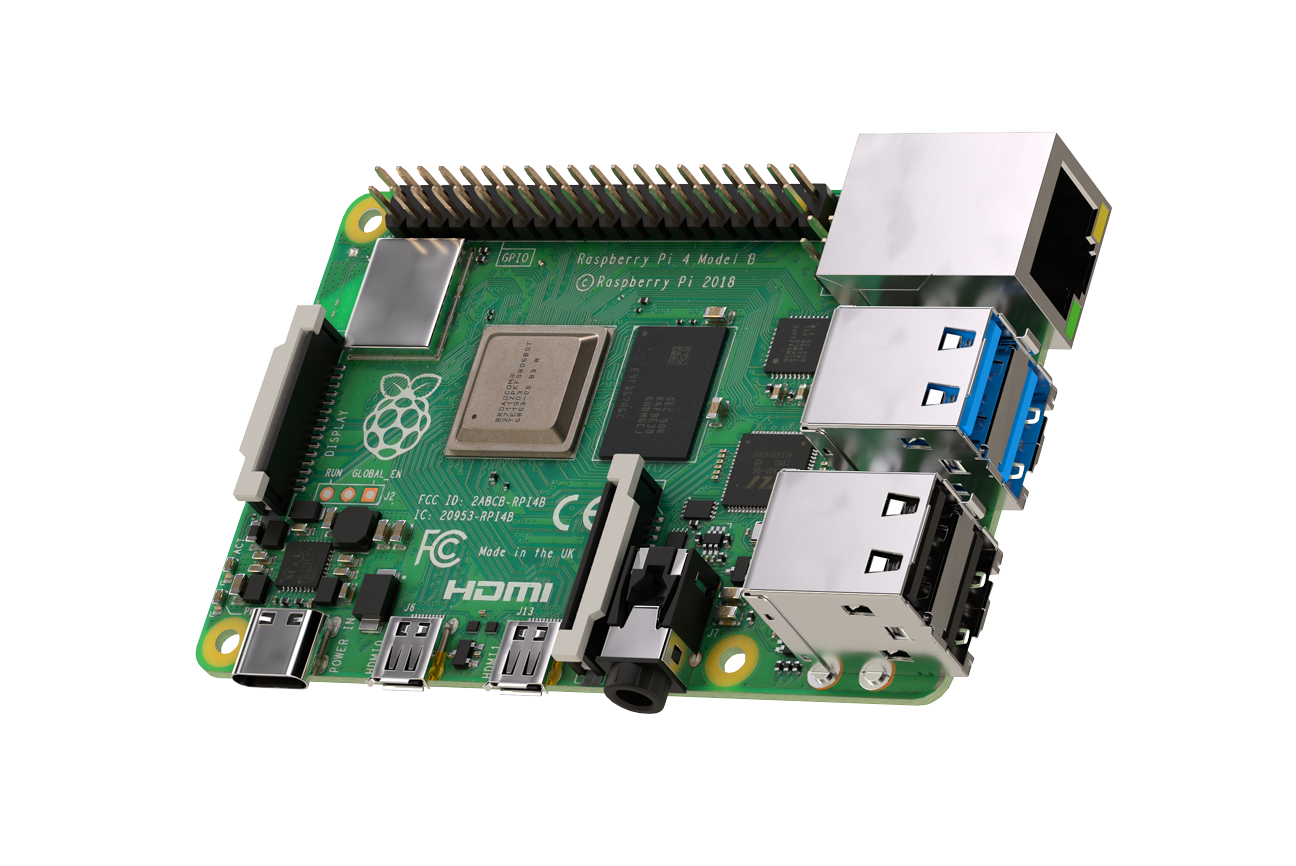
\includegraphics[width=0.8\textwidth]{rpi-4.png}
\captionsetup{justification=centering}
\caption{Raspberry Pi 4 B}
\end{figure}
\newline
\newline
Na laboratorijskim vježbama će se koristiti \textbf{Raspberry Bi 3 B}.
\newline
\newline
Tehničke karakteristike Raspberry Pi 3 B: \\
\textbf{SoC}: Broadcom BCM2837 \\
\textbf{CPU}: četverojezgreni ARM Cortex-A53, 1.2GHz \\
\textbf{GPU}: Broadcom VideoCore IV \\
\textbf{RAM}: 1GB LPDDR2 (900 MHz) \\
\textbf{Mreža}: 10/100 Ethernet, 2.4GHz 802.11n wireless \\
\textbf{Bluetooth}: Bluetooth 4.1 Classic, Bluetooth Low Energy \\
\textbf{Pohrana}: microSD \\
\textbf{GPIO}: 40-pin header, populated \\
\textbf{Priključci}: $4\times USB 2.0$, HDMI, 3.5mm analogni priključak,
 Ethernet, \textit{Camera Serial Interface} (CSI), \textit{Display Serial
 Interface} (DSI)
\begin{figure}%
\centering
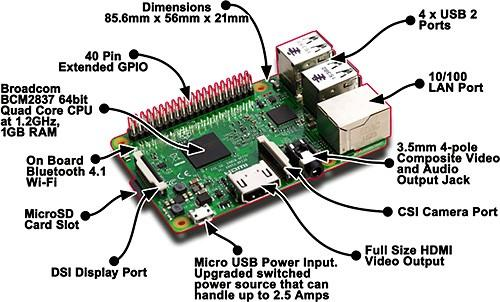
\includegraphics[width=0.8\textwidth]{rpi-3-details.jpg}
\captionsetup{justification=centering}
\caption{Raspberry Pi 3 detalji}
\end{figure}
\begin{figure}[h!]
	\centering
	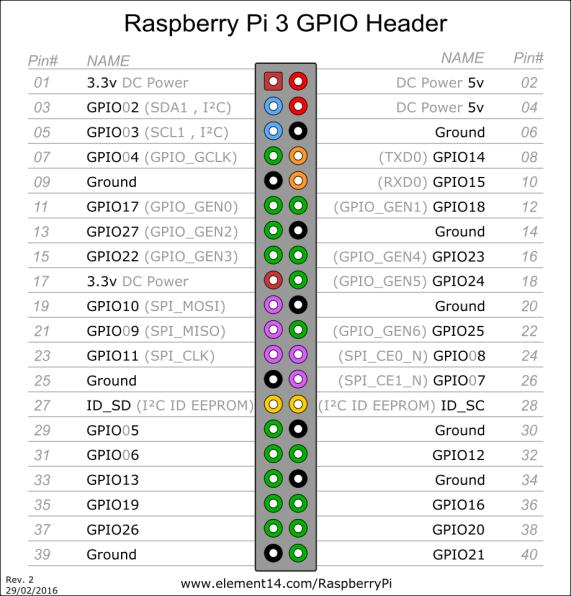
\includegraphics[width=0.8\textwidth]{rpi-3-pins.jpg}
	\captionsetup{justification=centering}
	\caption{Raspberry Pi 3 GPIO raspored}
	\label{fig:rpi-gpio}
\end{figure}

\clearpage
\section{Dodatna oprema}
Osim samog Raspberry Pi računala, potrebna je različita dodatna oprema ovisno
 o primjeni:

\begin{enumerate}
	\item napajanje 5V 2A, USB mikro priključak
	\item mikro SD memorijska kartica, kapaciteta min. 4GB klase A
	\item pretvornik USB na serijsku komunikaciju u obliku kabela (UART)
	\item pretvornik USB na Ethernet + Ethernet kabel
	\item dodatni uređaji za razvoj upravljačkih programa poput Nunchuk
		 upravljača.
\end{enumerate}

\begin{figure}%
    \centering
    \subfloat[Napajanje]{{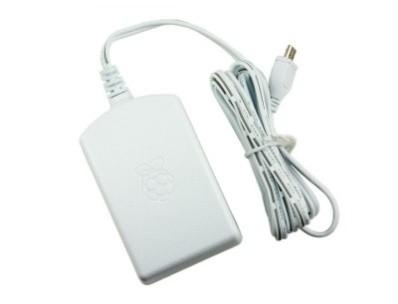
\includegraphics[width=4cm]{rpi-charger.jpg}}}%
    \subfloat[SD kartica]{{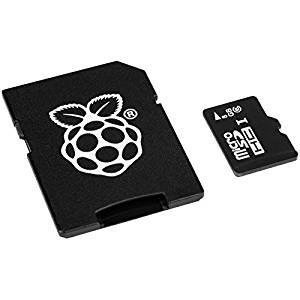
\includegraphics[width=4cm]{rpi-sdcard.jpg}}}%
    \subfloat[USB UART]{{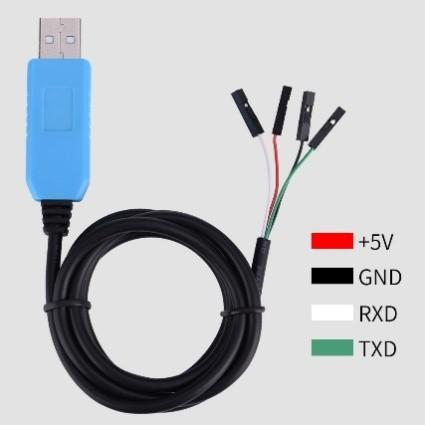
\includegraphics[width=4cm]{rpi-uart.jpg}}}%
    \qquad
    \subfloat[USB Ethernet]{{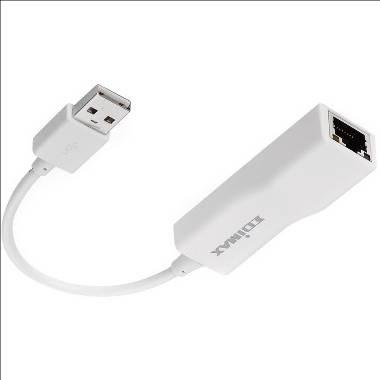
\includegraphics[width=4cm]{rpi-ethernet.jpg}}}%
    \subfloat[Nunchuk]{{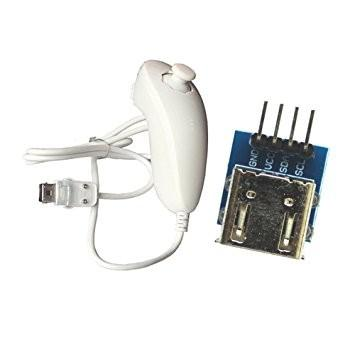
\includegraphics[width=4cm]{rpi-nunchuk.jpg}}}%
    \subfloat[Kućište]{{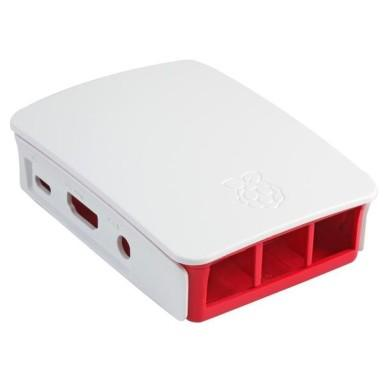
\includegraphics[width=4cm]{rpi-case.jpg}}}%
    \caption{Raspberry Pi dodatna oprema}%
    \label{fig:oprema1}%
\end{figure}

\section{Osnovne postavke}
Ako na razvojnom računalu nemate vaš repozitorij \texttt{embedded\_linux},
 najprije ga klonirajte odgovarajućom naredbom s vašeg Gitlab računa u vaš
 \texttt{home} direktorij. Pozicionirajte se u direktorij
 \texttt{/home/rtrk/embedded\_linux}. Zatim povucite moguće promjene iz
 izvornog repozitorija pomoću naredbe:
\begin{lstlisting}[language=bash]
git remote add upstream
	https://gitlab.com/rgrbic/embedded_linux
git fetch upstream
git merge upstream/master
\end{lstlisting}
Instalirajte potrebne alate na razvojno računalo:
\begin{lstlisting}[language=bash]
sudo apt-get install gcc-arm-linux-gnueabihf
\end{lstlisting}

\section{Buildroot}
\textit{Build} sustav je skup alata koji omogućuje automatizaciju procesa
 izgradnje Linuxa za ugradbene računalne sustave. Preciznije rečeno,
 \textit{build} sustavi omogućuju izgradnju \textit{toolchain} alata,
 \textit{bootloadera}, \textit{kernela} i \textit{root} datotečnog sustava na
 temelju izvornog koda. Neki od poznatijih build sustava su Buidroot, Yocto,
 PTXdist i OpenEmbedded. \\
\newline
Za potrebe izgradnje Linuxa za raspoloživo Raspberry Pi računalo koristit će se
 \textit{Buildroot} alat. Otvorite terminal i preuzmite \textit{Buildroot}
 pomoću naredbe:
\begin{lstlisting}[language=bash]
git clone https://github.com/buildroot/buildroot
\end{lstlisting}
Nakon što se postupak kloniranja na vaše razvojno računalo završi, uđite u
 kreirani direktorij:
\begin{lstlisting}[language=bash]
cd buildroot
\end{lstlisting}
Primijetit ćete da ovaj direktorij ima nekoliko poddirektorija (koristite
 naredbu \texttt{ls}) od kojih su najvažniji (detalji se mogu pogledati na\\
 \url{https://buildroot.org/downloads/manual/manual.html}):\\
\newline
 \texttt{dl}/: sadrži arhive od upstream projekata koje je Buildroot izgradio\\
\newline
 \texttt{output}/: ovdje se nalaze svi među i završni rezultati prevođenja
 izvora\\
\newline
\texttt{host}/: ovo su različiti alati koje zahtijeva \textit{Buildroot}, a
 koji se izvršavaju na host računalu, uključujući izvršne datoteke
 toolchaina (\textit{output/host/usr/bin})\\
\newline
\texttt{images}/: ovo je najvažniji direktorij jer se u njemu nalaze rezultati
izgradnje (ovisno što je odabrano kod konfiguracije \textit{buildroota} –
 bootloader, kernel i jedan ili više root datotečnih sustava)\\
\newline
\textit{staging}/: ovo je simbolička veza prema \textit{sysrootu toolchaina}\\
\newline
\textit{target}/: ovo je gotovo cjeloviti \textit{root} datotečni sustav
 (međutim nije namijenjen za korištenje kao \textit{root} datotečni sustav na
 target računalu)\\
\newline
\textit{configs}/: ovdje se nalaze predefinirane konfiguracije za različite
 ploče (npr. \textit{raspberrypi3\_defconfig})\\
\newline
\textit{boards}/: ovdje se nalaze različite skripte koje definiraju način
 generiranja slike cijelog sustava (sdcard.img), post build procedure i sl.\\
\newline
Iako se za potrebe izgradnje Linuxa pomoću Buildroota može koristiti\\
 \texttt{raspberrypi3\_defconfig} koji se dodatno modificira prema željama
 korisnika naredbom \texttt{make menuconfig|nconfig|xconfig}, u vježbi će se
 iskoristiti postojeća konfiguracija. Kopirajte
 \texttt{raspberrypi3\_ferit\_defconfig} datoteku iz repozitorija
 \texttt{/home/rtrk/embedded\_linux/LV2/resources} u direktorij
 \texttt{/home/rtrk/buildroot/configs}. Nadalje, kopirajte datoteke\\
 \texttt{post-build.sh} i \texttt{genimage-raspberrypi3.cfg} u direktorij\\
 \texttt{/home/rtrk/buildroot/board/raspberrypi}.\\
\newline
Učitajte danu konfiguraciju i
 provjerite što je sve uključeno u nju pokretanjem sljedećih naredbi u
 direktoriju \texttt{/home/rtrk/buildroot}:
\begin{lstlisting}[language=bash]
make raspberrypi3_ferit_defconfig
make menuconfig
\end{lstlisting}
Pokrenite izgradnju pomoću naredbe:
\begin{lstlisting}[language=bash]
make
\end{lstlisting}

Budući da alat \textit{Buildroot} prvi puta treba dohvatiti sve izvorne kodove
 različitih komponenata (\textit{toolchain}, \textit{bootloader}, \textit{kernel}
 i sl.), \textbf{izvođenje ove naredbe može potrajati, ovisno o brzini internet
 veze i brzini samog razvojnog računala}. U to vrijeme upoznajte se s Raspberry
 Pi i načinom izgradnje pojedinih komponenata Linuxa.
\newline
\newline
Pronađite na Raspberry Pi ploči 40 pinski header (Slika \ref{fig:rpi-gpio}) te
 identificirajte pinove za serijsku komunikaciju (RXD, TXD). Spojite pretvornik
 USB na serijsku vezu na način da povežete:\\
\newline
GND pretvornik $\leftrightarrow$ GND Raspberry Pi \\
TXD pretvornik $\leftrightarrow$ RX0 Raspberry Pi \\
RXD pretvornik $\leftrightarrow$ TX0 Raspberry Pi \\
\textbf{\textcolor{red}{(+5V pretvornika ne spajati na Raspberry Pi!)}} \\
\newline
Otvorite novi terminal. Instalirajte \textit{picocom} alat za serijsku
 komunikaciju pomoću naredbe:
\begin{lstlisting}[language=bash]
sudo apt-get install picocom
\end{lstlisting}
Testirajte serijsku vezu na način da spojite pretvornik na razvojno računalo. U
 terminalu izvršite naredbu:
\begin{lstlisting}[language=bash]
picocom -b 115200 /dev/ttyUSB0
\end{lstlisting}
Ako je pretvornik ispravno prepoznat, na ekranu će se ispisati "Terminal ready".
 Isključite USB pretvornik, u terminalu se treba prekinuti serijska veza. Ako
 želite napustiti \textit{picocom} bez isključivanja pretvornika iz USB-a,
 pritisnite Ctrl-a praćeno s Ctrl-x.
\newline
\newline
Nakon što se završi izgradnja Linuxa pomoću alata \textit{Buildroot}, u
 direktoriju \texttt{/home/rtrk/buildroot/output/images} nalazit će se sljedeće
 datoteke:
\newline
\dirtree{%
	.1 images.
	.2 bcm2710-rpi-3-b.dtb.
	.2 boot.vfat.
	.2 rootfs.ext2.
	.2 rootfs.ext4.
	.2 rpi-firmware.
	.3 bootcode.bin.
	.3 cmdline.txt.
	.3 config.txt.
	.3 fixup.dat.
	.3 start.elf.
	.3 overlays.
	.2 sdcard.img.
	.2 u-boot.bin.
	.2 zImage.
}%
Datoteka sdcard.img sadrži sve navedene dijelove Linuxa te ju je potrebno
 snimiti na mikro SD karticu. Ubacite mikro SD karticu u čitač memorijskih
 kartica i spojite ga na razvojno računalo (obično /dev/sdX gdje
 je X slovo a, b, c i sl.). Kopiranje ove datoteke na mikro SD karticu učinite
 naredbama:
\begin{lstlisting}[language=bash]
sudo dd status=progress if=sdcard.img of=/dev/sdx
sudo sync
\end{lstlisting}
Ako se pojave problemi prilikom zapisivanja datoteka na kraticu pomoću
 prethodnih naredbi, onda se preporuča instalacija alata \textit{GParted} koji
 je grafički alat za manipulaciju diskovima:
\begin{lstlisting}[language=bash]
sudo apt-get install gparted
\end{lstlisting}
Nakon instalacije pokrenite alat \textit{Gparted} iz Ubuntu grafičkog okruženja
 i obrišite sve particije koje se nalaze na vašoj mikro SD kartici
 (\textbf{\textcolor{red}{Oprez! Budite u potpunosti sigurni da brišete
 particije na mikro SD kartici, a ne nekog drugog medija za pohranu na računalu
 kao primjerice hard diska!}}).\\
\newline
Kada kopiranje datoteke uspješno završi, vaša mikro SD kartica će imati dvije
 particije pri čemu će se na prvoj particiji nalaziti datoteke potrebne za
 učitavanje OS-a (\textit{firmware}, \textit{bootloader} i sam \textit{kernel})
 dok će se na drugoj particiji nalaziti \textit{root} datotečni sustav.\\
Sigurno isključite čitač memorijskih kartica iz PC-a, izvadite mikro SD karticu
 i stavite ju u Raspberry Pi. Povežite PC i Raspberry Pi preko pretvornika USB
 na serijsku vezu, zatim spojite PC i Raspberry Pi preko USB to Ethernet
 pretvornika.\\
Otvorite serijsku vezu u novom terminalu na PC-u pomoću naredbe:
\begin{lstlisting}[language=bash]
picocom -b 115200 /dev/ttyUSB0
\end{lstlisting}
Spojite napajanje na Raspberry Pi. Nakon nekog vremena trebaju se pojaviti
 statusne poruke \textit{U-boot bootladera} u terminalu u kojem je otvorena
 serijska veza te naredbeni redak koji počinje s \texttt{U-boot>}. Pritisnite
 Enter kako biste zaustavili odbrojavanje odnosno \textit{autoboot}.

\section{U-boot konfiguracija}
Upisivanjem naredbe \texttt{help} u naredbeni redak \textit{U-boota} na ekranu
 će se ispisati popis dostupnih naredbi. Npr. izlistavanje svih varijable
 okruženja dobiva se naredbom:
\begin{lstlisting}[language=bash]
printenv
\end{lstlisting}
Promjena varijable okruženja provodi se pomoću naredbe \texttt{setenv} ili
 \texttt{editenv}. Na primjer:
\begin{lstlisting}[language=bash]
setenv boodelay 4
\end{lstlisting}
Pohranite okruženje nakon mijenjanja varijabli kako bi prilikom ponovnog
 pokretanja \texttt{U-boota} varijable imale postavljene vrijednosti. Pohranite
 okruženje na mikro SD karticu naredbom:
\begin{lstlisting}[language=bash]
saveenv
\end{lstlisting}
Kako bi se pokrenuo Linux potrebno je definiriati varijablu okruženja
 \texttt{bootargs} te definirati \texttt{bootcmd} koja će učitati
 \texttt{zImage} i odgovarajući \textit{device tree blob} na odgovarajuće
 adrese:
\begin{lstlisting}[language=bash]
setenv bootargs "8250.nr_uarts=1 root=/dev/mmcblk0p2
console=ttyS0,115200 rootfstype=ext4 elevator=deadline
fsck.repair=yes rootwait"

setenv bootcmd "fatload mmc 0:1 0x01000000 zImage;
fatload mmc 0:1 0x2000000 bcm2710-rpi-3-b.dtb;
bootz 0x01000000 - 0x2000000"
\end{lstlisting}
Spremite okruženje pomoću naredbe \texttt{saveenv} i zatim pokrenite Linux
 naredbom:
\begin{lstlisting}[language=bash]
run bootcmd
\end{lstlisting}
U terminalu ćete dobiti ispis o podizanju \textit{Linux} kernela i postavljanju
 \textit{root} datotečnog sustava. Po završetku podizanja dobit ćete redak za
 prijavu na sustav s imenom \texttt{buildroot}. Koristite korisničko ime
 \textbf{root}, \textbf{bez lozinke}.
\begin{lstlisting}[language=bash]
Welcome to Buildroot

buildroot login: root

buildroot:~#
\end{lstlisting}
Datotečni sustav sadrži osnovne naredbe u okviru \textit{BusyBoxa}. Pokušajte
 izlistati sadržaj direktorija i pronaći \textit{BusyBox}. Kada završite s
 radom, upišite naredbu
\begin{lstlisting}[language=bash]
poweroff
\end{lstlisting}
kako biste mogli sigurno isključiti ploču s napajanja. Ponovo uključite
 napajanje na ploči te kada započne odbrojavanje u \textit{U-bootu} zaustavite
 ga pritiskom na bilo koju tipku (u slučaju isteka vremena izvršit će se
 naredba \texttt{bootcmd}).

\section{Kopiranje datoteka korištenjem TFTP protokola i pokretanje sustava}
Kod razvoja Linux-a česte su promjene na slici kernela što zahtijeva kopiranje
 slike na mikro SD karticu. Kako bi se izbjeglo učestalo prebacivanje mikro SD
 kartice iz \textit{Raspberry Pi} u čitač memorijskih kartica i obrnuto, moguće
 je konfigurirati \textit{U-boot} i razvojno računalo tako da se datoteke
 prebacuju TFTP (engl. \textit{Trivial File Transfer Protocol}) protokolom.
 eajprije instalirajte TFTP server na razvojno računalo:
\begin{lstlisting}[language=bash]
sudo apt-get install tftpd-hpa
\end{lstlisting}
Mrežnim kabelom spojite \textit{Raspberry Pi} i razvojno računalo koristeći
 USB na Ethernet pretvornik. Spojite Raspberry Pi s razvojnim računalom pomoću
 pretvornika USB na serijsku vezu. Otvorite terminal i pokrenite
 \textit{picocom} serijski terminal odgovarajućom naredbom.
 Spojite napajanje na Raspberry Pi. Pritisnite tipku na računalu kako biste
 zaustavili automatsko podizanje sustava na Raspberry Pi. Na razvojnom računalu
 će se pojaviti nova mrežna veza. Postavite ovu mrežnu vezu kao što prikazuje
 slika \ref{fig:ubuntu-ethernet}. U kartici \textit{IPv4 Settings}, odaberite
 \textit{Manual} kao metodu kako biste omogućili statičku IP adresu, npr.
 192.170.0.1 (naravno, vodite računa da ova adresa pripada drugom mrežnom
 segmentu u odnosu na glavnu mrežu na koju je razvojno računalo već povezano).
 Za \textit{Netmask} postavite 24, a polje Gateway ostaviti prazno.
\begin{figure}[h!]
\centering
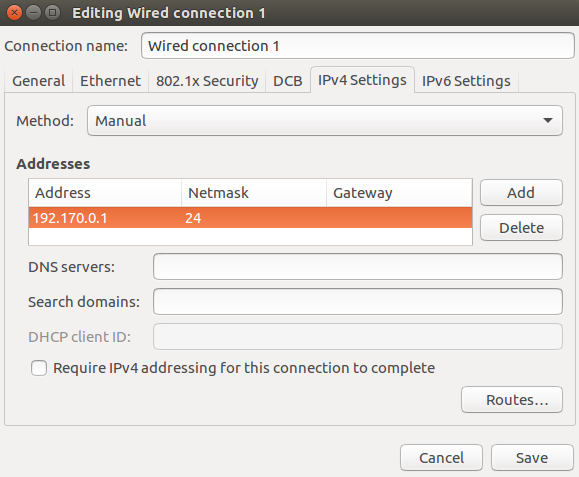
\includegraphics[width=0.8\textwidth]{ubuntu-ethernet.png}
\captionsetup{justification=centering}
\caption{Postavljanje nove mrežne veze koja odgovara USB na Ethernet
 pretvorniku}
\label{fig:ubuntu-ethernet}
\end{figure}
U U-Boot naredbenom retku potrebno je postaviti varijable okruženja koje
 odgovaraju IP adresi klijenta (Raspberry Pi) i servera (razvojno računalo),
 npr:
\begin{lstlisting}[language=bash]
setenv ipaddr 192.170.0.100
setenv serverip 192.170.0.1
\end{lstlisting}
Sačuvajte ove izmjene na mikro SD karticu naredbom:
\begin{lstlisting}[language=bash]
saveenv
\end{lstlisting}
Provjerite izmjene pomoću naredbe:
\begin{lstlisting}[language=bash]
printenv
\end{lstlisting}
Ispitajte radi li ispravno TFTP konekcija. Kreirajte malu tekstualnu datoteku u
 \texttt{/var/lib/tftpboot} naziva \texttt{file\_example.txt}. Pomoću
 naredbenog retka \textit{U-boota} izvršite sljedeću naredbu:
\begin{lstlisting}[language=bash]
tftp 0x01000000 file_example.txt
\end{lstlisting}
Ovom naredbom bi se trebala prebaciti datoteka \texttt{file\_example.txt} s
 razvojnog računala na Raspberry Pi ploču i to na memorijsku lokaciju
 \texttt{0x01000000} (ova lokacija pripada DRAM-u na ploči). Verificirajte ovaj
 upis čitanjem sadržaja s ove adrese:
\begin{lstlisting}[language=bash]
md 0x01000000
\end{lstlisting}
Provjeriti vezu možete i pomoću naredbe \texttt{ping}. Na Raspberry Pi (tj. u
 \textit{U-bootu}) izvršite naredbu:
\begin{lstlisting}[language=bash]
ping 127.0.0.1
\end{lstlisting}
Na razvojnom računalu izvršite naredbu:
\begin{lstlisting}[language=bash]
ping 127.0.0.1
\end{lstlisting}
Budući da je na Raspberry Pi mreža samo povremeno aktivna, pokušajte gore
 navedene naredbe izvršiti otprilike u isto vrijeme.
 U slučaju problema kod prebacivanja datoteke \texttt{file\_example.txt} i
 komunikacije: \\
\newline
1) Provjeriti IP adresu servera i klijenta koje su podešene u \textit{U-bootu}.
\newline
2) Pomoću naredbe \texttt{ls /var/lib/tftpboot} provjerite postoji li datoteka
 koju želite prebaciti.
\newline
3) Pokrenite ponovo servis \textit{tftpd-hpa} naredbom: \texttt{sudo service
 tftpd-hpa restart}.
\section{Postavljanje NFS Servera i datotečnog sustava}
Raspakirajte izgrađeni \textit{root} datotečni sustav u odgovarajući direktorij
 (pretpostavka je da se nalazite u vašem \textit{home} direktoriju):
\begin{lstlisting}[language=bash]
sudo tar xvjf buildroot/output/images/rootfs.tar.bz2 -C
embedded_linux/LV2/solutions/nfsroot
\end{lstlisting}
Promijenite prava u dobivenom direktoriju:
\begin{lstlisting}[language=bash]
sudo chown -R rtrk embedded_linux/LV2/solutions/nfsroot/root
\end{lstlisting}
Instalirajte NFS server pomoću naredbe:
\begin{lstlisting}[language=bash]
sudo apt-get install nfs-kernel-server
\end{lstlisting}
Izmijenite datoteku \texttt{/etc/exports} kao \textit{root} korisnik tako što
 ćete dodati narednu liniju:
\begin{lstlisting}[language=bash]
/home/rtrk/embedded_linux/LV2/solutions/nfsroot
<IP_adresa_rpi>(rw,no_root_squash,no_subtree_check)
\end{lstlisting}
pri čemu je \texttt{<IP\_adresa\_rpi>} podešena IP adresa \textit{Raspberry Pi}.
Ponovo pokrenite NFS server pomoću naredbe:
\begin{lstlisting}[language=bash]
sudo /etc/init.d/nfs-kernel-server restart
\end{lstlisting}
\section{Pokretanje sustava i učitavanje root datotečnog sustava preko NFS-a}
Pokrenite ploču do U-boot-a. Prije pokretanja jezgre potrebno je definirati
 koja se konzola koristi i koji će root datotečni sustav biti pokrenut preko
 NFS-a. Podesite U-boot \texttt{bootagrs} varijablu okruţenja na sljedeći
 način:
\begin{lstlisting}[language=bash]
setenv bootargs "root=/dev/nfs rw ip=<IP_adresa_rpi> 8250.nr_uarts=1
console=ttyS0,115200
nfsroot=<IP_adresa_pc>:/home/rtrk/embedded_linux/LV2/solutions/nfsroot"

saveenv
\end{lstlisting}
Ako kasnije želite promijeniti postavke, varijable možete mijenjati s:
\begin{lstlisting}[language=bash]
editenv bootargs
\end{lstlisting}
Sada prebacite sliku jezgre kroz TFTP:
\begin{lstlisting}[language=bash]
tftp 0x01000000 zImage
\end{lstlisting}
Potrebno je prebaciti i \textit{device tree blob}:
\begin{lstlisting}[language=bash]
tftp 0x2000000 bcm2710-rpi-3-b.dtb
\end{lstlisting}
Sada možete pokrenuti jezgru:
\begin{lstlisting}[language=bash]
bootz 0x01000000 - 0x2000000
\end{lstlisting}
Ako je sve u redu, pojaviti će se login prompt (korisnik: root, bez zaporke).
 Ako jezgra ne uspije podići mrežni datotečni sustav, pojavit će se poruke o
 greškama u terminalu. Pogledajte i NFS server poruke u \texttt{/var/log/syslog}
 na razvojnom računalu:
\begin{lstlisting}[language=bash]
cat /var/log/syslog
\end{lstlisting}
Moţete provjeriti radi li mreţni datotečni sustav na način da u root direktorij
 mrežnog datotečnog sustava dodate tekstualnu datoteku i u nju upišete
 proizvoljni tekst:
\begin{lstlisting}[language=bash]
sudo nano /home/rtrk/embedded_linux/LV2/solutions/nfsroot/root/proba.txt
\end{lstlisting}
Na Raspberry Pi bi se ista datoteka trebala nalaziti u \texttt{/root}
 direktoriju, npr. izvršite naredbu:
\begin{lstlisting}[language=bash]
cat /root/proba.txt
\end{lstlisting}
\section{Automatsko pokretanje sustava}
Kako biste izbjegli upisivanje istih naredbi svaki put kada se uključi ploča,
 možete koristiti U-Boot \texttt{bootcmd} varijablu:
\begin{lstlisting}[language=bash]
setenv bootcmd "tftp 0x01000000 zImage; tftp 0x2000000 bcm2710-rpi-3-b.dtb;
bootz 0x01000000 - 0x2000000"

saveenv
\end{lstlisting}
Slobodno ovo možete promijeniti po potrebi. Npr. ako želite vratiti pokretanje
 s mikro SD kartice:
\begin{lstlisting}[language=bash]
setenv bootargs "8250.nr_uarts=1 root=/dev/mmcblk0p2 console=ttyS0,115200
rootfstype=ext4 elevator=deadline fsck.repair=yes rootwait"

setenv bootcmd "fatload mmc 0:1 0x01000000 zImage; fatload mmc 0:1
0x2000000 bcm2710-rpi-3-b.dtb; bootz 0x01000000 - 0x2000000"

saveenv
\end{lstlisting}
\end{document}
